\chapter{Marco Teórico}
\label{ch:marco}

\section{NASA engineering lifecycle}
The NASA reference lifecycle progresses from Pre-Phase A (Concept Studies), through A (Concept and Technology Development) and B (Preliminary Design and Technology Completion), to C (Final Design and Fabrication). Requirements, design and technical management processes recur as products mature. Phase C normally includes detailed design, hardware fabrication and software coding. CDR occurs during C before deliverable coding. SIR occurs at its end to assess integration readiness \citep[Secs.~2.2--2.3, 3.3--3.6 and Table~6.7-1]{nasa2016systems}.

\section{Concept of Operations}
A Concept of Operations is a high-level description of how a system will be used to meet stakeholder expectations, usually in a time sequence. It provides an operational perspective that guides requirements and architecture development \citep[Sec.~4.1.1.2.4 and Appendix~B]{nasa2016systems}.

\section{Verification and validation}
Verification establishes conformity to applicable requirements. Validation assesses suitability for stakeholder expectations and ConOps in the intended environment. Validation may use models under representative simulated conditions. Analysis is a valid validation method. Requirements validation also checks correctness, feasibility, consistency, verifiability and stakeholder suitability. Model calibration adjusts parameters against data. Independent validation data, assumptions, uncertainty and the intended validity domain are needed to assess a model's credibility \citep[Secs.~2.4, 4.2 and~5.3--5.4]{nasa2016systems}\citep[pp.~7--9]{handpicked-0001}.

\section{Model-, software-, processor-, and hardware-in-the-loop}

MIL executes a modeled controller with a modeled EPS plant. SIL executes control/interface code on a test processor (not the processor meant to be used in the final system) with simulated inputs and outputs. PIL executes code on the target processor. HIL couples simulation with physical hardware. MIL and SIL can provide evidence about the assessed models and code. They establish no target processor power performance by themselves \citep{handpicked-0001,review-0573}.

\section{Model-based Systems Engineering}
Buruso et al. describe model-based systems engineering (MBSE) as the use of a shared system model across engineering disciplines and throughout the system lifecycle, from identifying stakeholder needs to development and operations \cite{buruso2026modelbased}.
Such models can capture functional, logical, and physical characteristics at different levels of design detail.
They can also support simulation, comparison of candidate solutions, and data exchange across tools and engineering roles \cite{buruso2026modelbased}.
Potential benefits of the adoption of MBSE include lower documentation effort and development cost, better system understanding and collaboration, earlier fault detection, and reduced technical risk \cite{buruso2026modelbased}.

\section{The Object-Oriented Systems Engineering Methodology}
OOSEM is a top-down, scenario-driven MBSE method that serves to analyze, specify, design, and support the verification of systems. Its primary output is an integrated system model with consistent views of behavior, structure, properties, and requirements traceability. Its specification and design activities progress from stakeholder needs and black-box system requirements to logical and physical architectures. Engineering analysis, trade studies, and traceability span these activities. The activities are tailored and iterated rather than executed as fixed sequential phases \citep{friedenthal2014practical}.

Figure~\ref{fig:systems-engineering-technical-processes} summarizes the systems engineering technical process. Stakeholder needs inform system specification and design. Component requirements guide component design, implementation, and test. Verified components feed system integration and test. Feedback from component work and integration returns to system specification and design \citep[Fig.~1.1]{friedenthal2014practical}. OOSEM implements system specification and design and supports integration and verification through model-based test cases. The development process can be applied recursively at successive levels of the system hierarchy \citep[Sec.~17.1.2]{friedenthal2014practical}.

\begin{figure}[htbp]
    \centering
    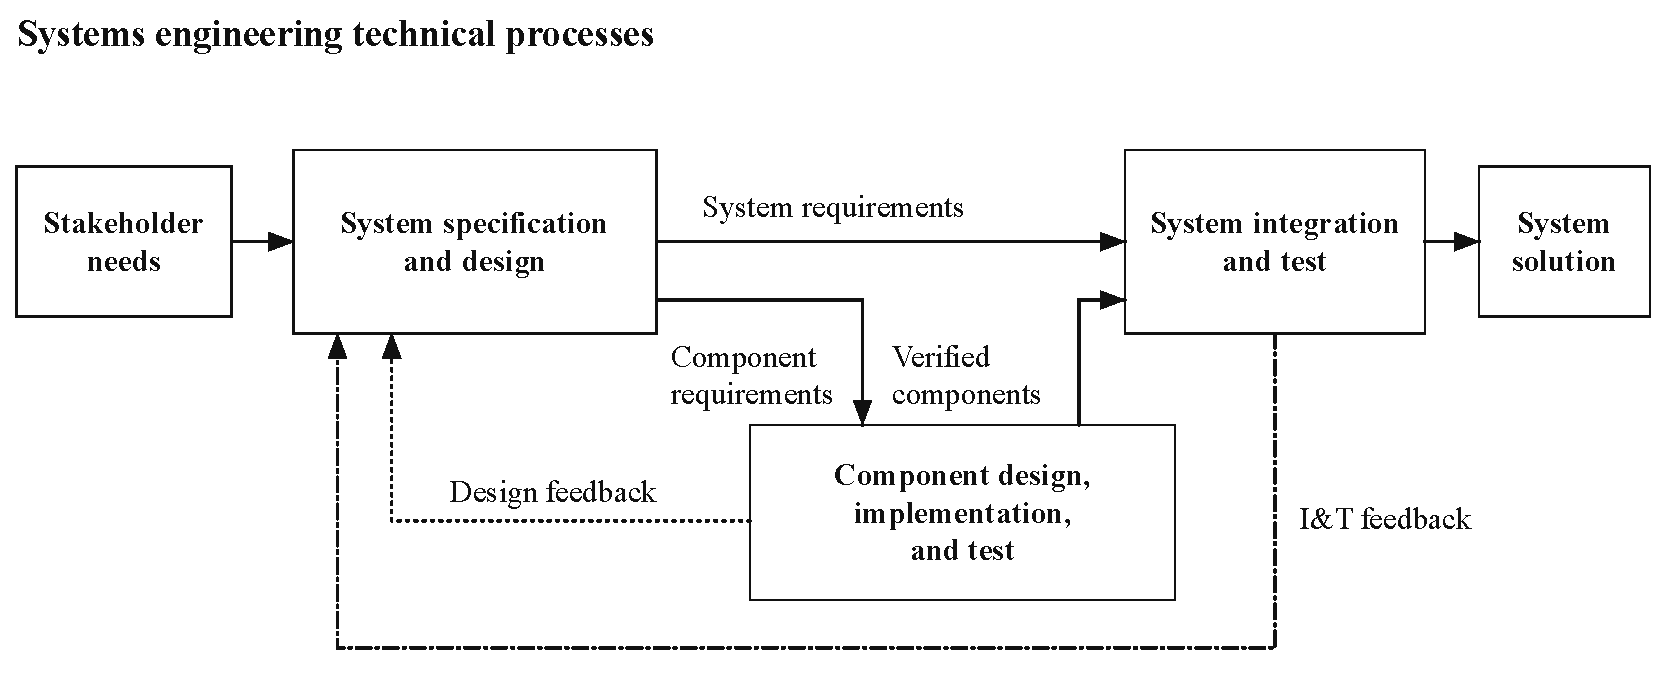
\includegraphics[width=\linewidth]{fig/systems-engineering-technical-processes.pdf}
    \caption[Simplified systems engineering technical processes.]{Simplified systems engineering technical processes. Solid arrows carry forward exchanges. Dotted arrows carry design feedback. Dash-dot arrows carry integration and test feedback. Adapted from \citet[Fig.~1.1]{friedenthal2014practical}.}
    \label{fig:systems-engineering-technical-processes}
\end{figure}

\paragraph{Stakeholders.}
In OOSEM, a stakeholder is a person or organization with an interest in the system across its lifecycle. A stakeholder role identifies whose concerns must be addressed \citep[Secs.~17.3.2 and 17.3.5]{friedenthal2014practical}.

\paragraph{Operational domain as-is and to-be, and enterprise.}
An operational domain provides the context for the system of interest. It contains the operational system, the users and external systems with which it interacts, and the relevant environment. An as-is domain characterizes the current context sufficiently to understand stakeholder concerns. A to-be domain describes the intended context after the mission need is addressed. Within a domain, an enterprise is an aggregation of systems and users that collaborate to achieve a set of mission objectives. It contains the system of interest and the supporting participants needed to accomplish those objectives, while other actors and environmental elements may remain external to it \citep[Sec.~17.3.2]{friedenthal2014practical}.